\chapter{Zerocoin e Zerocash}
L’anonimato nelle transazioni finanziarie rappresenta un diritto fondamentale per molti utenti di criptovalute. Sappiamo che Bitcoin offre solamente pseudonimità, con transazioni potenzialmente tracciabili attraverso tecniche di analisi del grafo e clustering degli indirizzi. 

In questo contesto, Zerocoin e la sua evoluzione Zerocash emergono come protocolli particolarmente significativi, rappresentando non semplici miglioramenti ma vere rivoluzioni concettuali nell’approccio all’anonimato, attraverso l’utilizzo innovativo di primitive crittografiche avanzate.

\section{Zerocoin}
L'idea dello Zerocoin può essere spiegata attraverso una metafora di una bacheca pubblica condivisa. Supponiamo che un utente desideri creare uno Zerocoin, questo utente spende un qualcosa detto \textbf{base coin} e crea un \textbf{numero seriale} di cui fa un \textbf{commitment} cioè il seriale è in una busta opaca. 

Gli altri utenti controllano che ciò che ha speso sia effettivamente valido e controllano anche che il commitment sia valido. 

A questo punto supponiamo di voler spendere questo Zerocoin, l'utente produrrà una Zero Knowledge che dimostri:
\begin{itemize}
    \item Il fatto che l'utente conosca il commitment $C$.
    \item Il fatto che lei conosca (senza rivelarlo) il valore $r$ tale che $c$ esponga $s$. 
\end{itemize}
Questo tipo di commitment è del tipo $C= g^S h^r$ e l'utente, per spendere la moneta, mostrerà $S$ e mostrerà in Zero knowledge che con questo S è stato creato C con un certo $r$ che solo lei conosce.

Questa prova verrà fatta tramite una prova \textbf{non interattiva}, generando $c = H(R || \dots)$ e, poiché l'hash non è prevedibile, allora ci si può mostrare. Inoltre, poiché $S$ viene mostrato, allora quello Zerocoin non è più spendibile poiché presente nella blockchain.

\subsection{Minting}
Cerchiamo di formalizzarlo correttamente adesso. La coniazione rappresenta la fase iniziale nel ciclo di vita di uno Zerocoin, dove un utente converte un'unità di valuta base in uno Zerocoin. Il processo si articola nei seguenti passaggi:

\begin{enumerate}
    \item \textbf{Generazione del seriale:} L'utente genera un numero seriale casuale $S$ che identificherà univocamente la moneta, mantenendolo inizialmente segreto.
    \item \textbf{Calcolo del commitment:} Viene calcolato un commitment crittografico $C = \text{Com}(S, r)$ utilizzando il numero seriale $S$ e un valore casuale $r$ (\textit{randomness}). Il commitment funziona come una cassaforte digitale con le proprietà di:
    \begin{itemize}
        \item \textbf{Hiding}: impossibilità di estrarre $S$ a partire da $C$;
        \item \textbf{Binding}: impossibilità di cambiare $S$ una volta pubblicato $C$, permettendo di verificare successivamente che $C$ contenga effettivamente quel determinato $S$.
    \end{itemize}
    \item \textbf{Pubblicazione}: L'utente pubblica il commitment $C$ sulla blockchain insieme a un'unità della valuta base tramite una transazione di tipo "Mint".
    \item \textbf{Verifica}: I nodi della rete verificano che il commitment sia correttamente formato e che l'unità di valuta base sia autentica.
\end{enumerate}

Gli Zerocoin vengono emessi in \textbf{denominazioni standard}, creando un "anonymity set" omogeneo che impedisce il tracciamento basato sui valori delle transazioni.

A livello di protocollo, Zerocoin è anonimo, tuttavia, tramite side channel, è possibile rompere l'anonimato.


\subsection{Redeeming}
Il processo di riscatto si sviluppa nel seguente modo:

\begin{enumerate}
    \item \textbf{Identificazione dei commitment:} L'utente esamina la blockchain per identificare tutti i commitment Zerocoin registrati, costruendo l'insieme $(C_1, C_2, \dots, C_n)$ che include il proprio commitment.
    \item \textbf{Generazione della prova:} Genera una prova zero-knowledge non interattiva $\pi$ che dimostra due fatti: 
    \begin{enumerate}
        \item l'utente conosce un commitment $C$ presente nell'insieme pubblico $C_1 \dots C_n$;
        \item l'utente conosce un valore $r$ tale che $C$ si apre correttamente sul numero seriale $S$ che sta per essere rivelato.
    \end{enumerate}
    \item \textbf{Pubblicazione della transazione:} Pubblica sulla blockchain una transazione di spesa contenente la coppia $(S, \pi)$, composta dal numero seriale e dalla prova zero-knowledge.
    \item \textbf{Verifica:} I validatori verificano che il numero seriale non sia già stato utilizzato (prevenendo la doppia spesa) e che la prova $\pi$ sia matematicamente valida.
\end{enumerate}
La proprietà "zero-knowledge" della prova garantisce che, pur dimostrando la validità del riscatto, non venga rivelato quale specifico commitment l'utente stia utilizzando. Sebbene tutte le transazioni siano pubbliche, risulta matematicamente impossibile collegare il numero seriale rivelato a uno specifico commitment originale.

\subsection{Limiti Tecnici}
I commitment sono pubblicati potenzialmente da tutti gli utenti e sappiamo che più è grande lo statement, più è grande la prova in Zero Knowledge. Nel nostro caso, la prova che dovremmo mostrare è che
\[(C=C_1) \cup (C=C_2) \cup \dots (C = C_n)\]

E questo, a livello computazionale è insostenibile e irrealizzabile in pratica.

\subsection{Accumulatori crittografici}
La funzione degli accumulatori essenziale è trasformare l'insieme di commitment $(C_1, \dots, C_n)$ in un singolo digest crittografico $A$ la cui dimensione rimane costante indipendentemente dalla cardinalità dell'insieme.

Le proprietà fondamentali di un accumulatore crittografico includono:
\begin{itemize}
    \item \textbf{Compattezza:} La dimensione dell'accumulatore rimane costante indipendentemente dal numero di elementi accumulati.
    \item \textbf{Efficienza di verifica:} La verifica dell'appartenenza di un elemento all'accumulatore ha complessità computazionale sublineare (idealmente costante o logaritmica) rispetto alla dimensione dell'insieme.
    \item \textbf{Unidirezionalità:} È computazionalmente intrattabile derivare gli elementi originali dal valore dell'accumulatore.
    \item \textbf{Resistenza alle collisioni:} È computazionalmente intrattabile trovare un elemento valido che non è stato incluso nell'accumulatore.
\end{itemize}

Nel contesto di Zerocoin, gli accumulatori permettono di riformulare la prova di appartenenza in modo drammaticamente più efficiente. Anziché dimostrare una disgiunzione su tutti i commitment, l'utente deve semplicemente provare di conoscere un "testimone"(\textit{witness}) $w$ che attesti l'appartenenza del proprio commitment $c$ all'accumulatore $A$.

\subsubsection{RSA}
Prima di andare avanti, è necessario discutere di RSA e spiegarlo semplicemente. Sia N il prodotto di due primi $p,q$ e $e$ un esponente pubblico. La funzione RSA è definita come:
\[RSA[N, e](x) = x^e \mod N\]
Questa è la prima \textbf{funzione trapdoor} per cui, dati $e,N$ e $y =x^e \mod N$, è possibile ritrovare x solo se si ha la conoscenza di $p,q$.
Per estrarre x utilizziamo l'algoritmo esteso di Euclide con input la $p, q$ ed $e$. In sostanza questo algoritmo ci permette di estrarre radici $e-esime$. 

A partire dallo stesso N, si possono creare più y utilizzando diversi e.

RSA è uno strumento molto utile che serve anche per fare le firme blind ecc. 
\subsection{Implementazione degli Accumulatori}
La costruzione di questi accumulatori è fatta mediante l'uso di diversi algoritmi:
\begin{itemize}
    \item \textbf{Setup}: Viene generato $N = pq$ e $w$ che è un elemento non nullo minore di $N$. 
    \item \textbf{Accumulate(params, $(c_1,\dots, c_n)$)}: Qui, quello che vogliamo fare è il \textbf{commitment di tanti valori in un insieme}. Per farlo, calcoliamo $A = u^{c_1 \cdot \dots \cdot c_n} \mod N$. $A$ sarà un elemento nell'ordine di N poiché vi è il modulo.
    \item \textbf{GenWitness(params, v, $(c_1,\dots, c_n)$)}: Questo genererà un testimone che dimostrerà che il nostro c è un elemento in quell'insieme. Per fare una cosa di questo tipo, supponiamo $ c \in V = (c_1,\dots, c_n)$ e se $v \in V$ allora calcoliamo un altro accumulatore $Accumulate(params, V-\{v\}) = w$.
    \item \textbf{Acc.Verify(params, s, v, w, A)}: Banalmente adesso calcoliamo $A' = w^v \mod N$ e se $A == A'$, allora la cosa è corretta.  
\end{itemize}
Questa cosa è sicura perché chi fa il setup elimina $p, q$ e, dunque, nessuno conosce la fattorizzazione di $N$ e, dunque, l'unico modo per calcolare la prova è o farlo correttamente o estrarre la fattorizzazione ma ciò è impossibile.

\subsection{Integrazione in Zerocoin}
Nel contesto di Zerocoin, l'integrazione degli accumulatori RSA permette di riformulare le prove di riscatto in modo sostanzialmente più efficiente. La prova di riscatto si trasforma in una dimostrazione zero knowledge strutturata come segue:

\begin{equation}
    \text{``Conosco } (c, w, r) \text{ tali che:''}
\end{equation}

\begin{itemize}
    \item $c$ è un commitment valido incluso nell'accumulatore $A$ (verificabile attraverso il testimone $w$)
    \item $c$ si apre correttamente sul numero seriale $S$ dichiarato, ovvero $c = H(S, r)$
\end{itemize}

Questa formulazione comporta diversi vantaggi critici:

\begin{itemize}
    \item \textbf{Efficienza computazionale:} La generazione e verifica della prova hanno complessità costante rispetto al numero di commitment nel sistema.
    \item \textbf{Dimensione della prova:} La prova stessa ha dimensione costante (tipicamente alcuni kilobyte), indipendentemente dalla dimensione dell'insieme dei commitment.
    \item \textbf{Scalabilità:} Il sistema può supportare un numero arbitrariamente grande di commitment senza degradazione significativa delle prestazioni.
\end{itemize}

\subsection{Sfide di Integrazione e Problematiche}

Nonostante l'eleganza teorica, l'integrazione di Zerocoin nel protocollo Bitcoin presenta ostacoli tecnici e fiduciari che ne hanno impedito l'adozione su larga scala nella rete principale. Le criticità si possono riassumere in tre punti fondamentali:

\begin{itemize}
    \item \textbf{Limitazioni di Bitcoin Script:} Bitcoin utilizza un linguaggio di scripting non completo (non Turing-completo) e volutamente limitato per ragioni di sicurezza e prevedibilità. Verificare le operazioni matematiche complesse necessarie per gli accumulatori RSA e per le prove Zero-Knowledge richiederebbe l'introduzione di nuovi codici operativi (\textit{opcodes}) estremamente pesanti. Attualmente, Bitcoin Script non è in grado di processare tali verifiche in modo nativo.
    
    \item \textbf{Divergenza nei Meccanismi di Verifica:} Mentre Bitcoin si affida alle firme digitali \textbf{ECDSA} (o Schnorr) per autorizzare il trasferimento di UTXO, Zerocoin sostituisce il concetto di firma con una \textbf{dimostrazione Zero-Knowledge}. Questo cambio di paradigma richiederebbe una modifica strutturale al modo in cui i nodi validano le transazioni: non si tratterebbe più di verificare la proprietà di una chiave, ma la correttezza di una prova di conoscenza relativa a un accumulatore.
    
    \item \textbf{Il problema del Trusted Setup (TTP):} Come discusso nella sezione relativa a RSA, il sistema si basa su un modulo $N = p \cdot q$. Per garantire che nessuno possa falsificare monete dal nulla, è necessario che i fattori primi $p$ e $q$ vengano distrutti immediatamente dopo la generazione di $N$. Questo processo richiede l'esistenza di una \textbf{Trusted Third Party} (TTP) che esegua il setup iniziale. In un ecosistema decentralizzato come quello delle criptovalute, l'esistenza di parametri che richiedono fiducia in un ente centrale (o in un evento di generazione "sacro") rappresenta un punto di fallimento e una contraddizione filosofica rispetto ai principi di Bitcoin.
\end{itemize}

Queste problematiche hanno portato la ricerca crittografica verso soluzioni più efficienti e meno dipendenti da setup fiduciari, culminando nello sviluppo di Zerocash.

\section{Zerocash}
Zerocash, presentato nel 2014 al simposio Usenix Security da E. Ben-Sasson et al., rappresenta un'evoluzione fondamentale rispetto a Zerocoin, superandone le limitazioni strutturali e introducendo un paradigma completamente nuovo per la privacy nelle criptovalute. A differenza di Zerocoin, che operava come un'estensione del protocollo Bitcoin richiedendo una valuta base, Zerocash è stato concepito come un sistema autonomo e completo, svincolato dalla necessità di una valuta sottostante.

Le innovazioni principali di Zerocash rispetto al suo predecessore sono duplici:
\begin{itemize}
    \item \textbf{Efficienza crittografica}: l'implementazione di primitive crittografiche sostanzialmente più efficienti per la generazione e verifica delle prove di conoscenza zero. Queste sono le zk-SNARKs che permettono l'uso di prove zero knowledge con statement parecchio lunghi ma dando in output risultati piccoli.
    \item \textbf{Architettura indipendente}: lo sviluppo di un'architettura che funziona interamente attraverso transazioni anonime, eliminando il vincolo di una valuta base esterna come avveniva per Zerocoin.
\end{itemize}

\subsection{Il problema del Trusted Setup in Zerocash}

Nonostante i significativi avanzamenti tecnici, Zerocash eredita e per certi versi amplifica la problematica del "setup fidato" già presente in Zerocoin. La generazione dei parametri pubblici per le prove zk-SNARK richiede input casuali e segreti che devono essere irrecuperabilmente distrutti dopo la creazione dei parametri pubblici.

Questa fase rappresenta un punto critico nel sistema: chiunque entrasse in possesso di questi valori segreti potrebbe compromettere irrimediabilmente l'intero protocollo, generando fondi dal nulla senza possibilità di rilevamento. Le implicazioni di questa vulnerabilità sono particolarmente severe:

\begin{itemize}
    \item \textbf{Compromissione totale}: A differenza di Zerocoin, dove la compromissione avrebbe consentito principalmente la falsificazione di prove, in Zerocash comprometterebbe l'intero sistema monetario, permettendo la creazione illimitata di valuta.
    \item \textbf{Difficoltà di rilevazione}: La natura delle prove rende potenzialmente impossibile rilevare l'avvenuta compromissione, in contrasto con altri attacchi crittografici che lasciano tracce identificabili.
    \item \textbf{Complessità della cerimonia}: La generazione dei parametri richiede una "cerimonia multi-parte" estremamente sofisticata, in cui diversi partecipanti contribuiscono alla creazione dei parametri in modo che tutti debbano essere compromessi per danneggiare il sistema.
\end{itemize}

Questa problematica rappresenta il principale ostacolo all'adozione di Zerocash e ha stimolato ulteriori ricerche sulla generazione di parametri in contesti a fiducia distribuita o minimizzata.

\section{Il Continuum dell'Anonimato nelle Criptovalute}

Zerocash si posiziona all'estremità del continuum dell'anonimato nelle criptovalute, rappresentando il massimo livello di privacy attualmente raggiungibile. Analizzando i diversi approcci alla privacy nelle criptovalute, è possibile identificare cinque livelli progressivi di anonimato, come illustrato nella tabella seguente:
\begin{figure}[H]
    \centering
    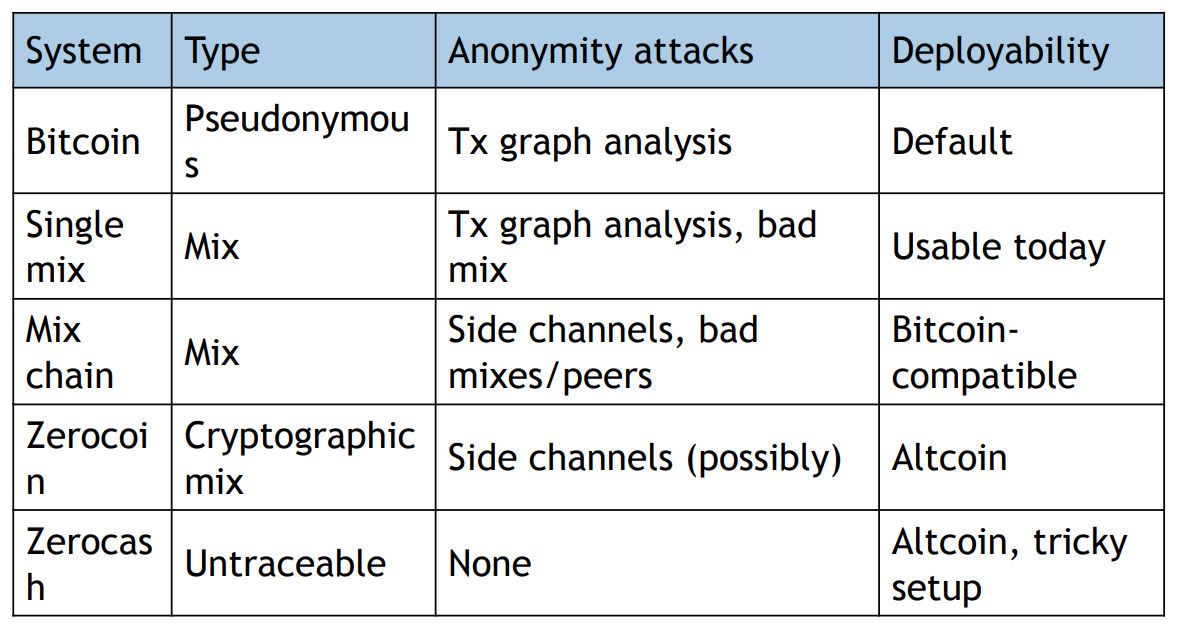
\includegraphics[width=0.6\linewidth]{Images/capitolo_5/lv_anonimato.png}
\end{figure}
Questa progressione evidenzia il trade-off fondamentale tra livello di anonimato e complessità implementativa/computazionale, con Zerocash che rappresenta la frontiera attuale della privacy crittografica, al costo di significative sfide tecniche e di adozione.